% Template: LaTeX file for ICMC 2009 papers, with hyper-references
%
% derived from the DAFx-06 templates
%
% 1) Please compile using latex or pdflatex.
% 2) Please use figures in vectorial format (.pdf); .png or .jpg are working otherwise 
% 3) Please use the "papertitle" and "pdfauthor" commands defined below

%------------------------------------------------------------------------------------------
\documentclass[twoside,10pt]{article}
\usepackage{icmc2009,amssymb,amsmath} 
%\setcounter{page}{1}

\usepackage{mathptmx} 

%____________________________________________________________
%  !  !  !  !  !  !  !  !  !  !  !  ! user defined variables  !  !  !  !  !  !  !  !  !  !  !  !  !  !
%==== set the title ====
\def\papertitle{DBAP - Distance-based amplitude panning}
%\def\papertitle{}	%-- should be empty for the submission anyway!

%==== 1st submission: author name and affiliation are empty for anonymous submission ====
%\def\paperauthorA{} 
%\affiliation{}{}


%==== final submission: author name and affiliation ====
%---- uncomment 1 to 4 lines, for 1 to 4 authors
\def\paperauthorA{Trond Lossius}
\def\paperauthorB{Pascal Baltazar}
\def\paperauthorC{Th\'eo de la Hogue}
%\def\paperauthorD{Fourth Author}

%%---- set correspnding affiliation data for...
%%-- 1 author
%\affiliation{\paperauthorA}
%  {School\\ Department, City, Country \\ {\tt \href{mailto:email@domain.icmc}{email@domain.icmc}}}

%%-- 2 authors with same affiliation
%\affiliation{\paperauthorA, \paperauthorB}
%  {School\\ Department, City, Country \\ {\tt \href{mailto:email@domain.icmc}{email@domain.icmc}}}

%-- 2 authors with different affiliations
%\twoaffiliations{\paperauthorA}{School\\ Department}
%  {\paperauthorB}{Company\\ Address}

%%-- 3 authors with different affiliations
\threeaffiliations{\paperauthorA}{BEK\\C. Sundtsgt. 55\\5004 Bergen\\Norway\\trond.lossius@bek.no}
  {\paperauthorB}{GMEA\\4 rue Sainte Claire\\81000 Albi\\France\\pb@gmea.net}
  {\paperauthorC}{GMEA\\4 rue Sainte Claire\\81000 Albi\\France\\theod@gmea.net}

%%-- 4 authors with different affiliations
%\fouraffiliations{\paperauthorA}{School A\\ Department X}
%  {\paperauthorB}{Company\\ Address}
%  {\paperauthorC}{School B\\ Department Y}
%  {\paperauthorD}{School C\\ Department Z}

%  ^  ^  ^  ^  ^  ^  ^  ^  ^  ^ user defined variables  ^  ^  ^  ^  ^  ^  ^  ^  ^  ^  ^  ^ 
%------------------------------------------------------------------------------------------

%%-- if using .ps or .eps figure files, they will be converted on the fly
%%-- RMK: for faster LaTeX runs, use it only once after adding new \includegraphics[]{} cmds
%\usepackage{epstopdf}	 

%---- the hyperref package must be last to properly work
\usepackage[pdftex,
       pdftitle={\papertitle},
	pdfauthor={\paperauthorA},
	colorlinks=false,bookmarksnumbered,pdfstartview=XYZ]{hyperref}
%\pdfcompresslevel=9
\usepackage[pdftex]{graphicx}	% for compatible graphics with hyperref
\usepackage[figure,table]{hypcap}	% corrects the hyper-anchor of figures/tables

\title{\papertitle}

%------------------------------------------------------------------------------------------
\begin{document}

\DeclareGraphicsExtensions{.png,.jpg,.pdf} % used graphic file format for pdflatex
    
\maketitle




%%%%%%%%%%%%%%%%%%%%%%%%%%%%%%%%%%%%%%%%%%%%%%%%%%%%%%%%%
%
% Abstract
%
%%%%%%%%%%%%%%%%%%%%%%%%%%%%%%%%%%%%%%%%%%%%%%%%%%%%%%%%%




\begin{abstract}
The abstract should be placed at the top left column and should contain
about 150 words.
\end{abstract}








%%%%%%%%%%%%%%%%%%%%%%%%%%%%%%%%%%%%%%%%%%%%%%%%%%%%%%%%%
%
% Introduction
%
%%%%%%%%%%%%%%%%%%%%%%%%%%%%%%%%%%%%%%%%%%%%%%%%%%%%%%%%%


\section{Introduction}\label{sec:introduction}

The use of multichannel and surround sound reproduction is getting ever more common, for consumer applications as well as musical and artistic purposes. A number of techniques exist for virtual positioning of sound sources using an array of loudspeakers. A common assumption of techniques for spatialisation is that the position of the listener is known and fixed, and the speakers are surrounding the listener either on a two-dimensional ring or a three-dimensional sphere. Examples of such speaker layouts and spatialisation techniques are stereo panning, 5.1-channel surround \cite{ITU:1993_surround_5:1}, further extended industrial multichannel configurations \cite{Rumsey:2001spatial_audio}, vector-based amplitude panning (VBAP) \cite{Pulkki:1997vbap} and first and higher-order ambisonics \cite{Gerzon:1974surround, Poletti:2000holographic_sound}.

Wave field synthesis (WFS) is a noticeable exception to the above sweet spot restriction, reproducing signals resulting in a large listening area. The spatial properties of the acoustical scene can be perceived correctly by an arbitrary large number of listeners regardless of their position inside this area \cite{Spors:2004sound_field_synthesis}.

For musical and artistic use a number of practical limitations tend to restrict what spatialisation techniques are feasible to use.

Unless working on a site providing a permanent setup for wave field synthesis, the high number of loudspeakers required might render WFS impractical for financial reasons as well as time constraints.

For real-time music and sound purposes the relative low CPU requirements of matrix-based spatialisation techniques seems to make them popular choices, and VBAP as well as first and higher order ambisonics are readily available for use in common software environments for real-time processing such as Max/MSP \cite{Pulkki:2000vbap_max, Schacher:2006ambi_max, Neukom:2008ambipan}.

The requirements imposed by VBAP and ambisonics with respect to listeners being restricted to a relatively small listening area surrounded by loudspeakers might be impractical or even undesired in practical applications. In a concert situation ideally all of the audience should have a detailed impression of the spatial content of the music, not only the ones sitting at the middle of the hall. In a sound installation context one might want the audience to be able to move around the space \cite{lossius:2008installations}. And finally, for practical and/or artistic reasons it might not be possible or desired to have loudspeakers arranged in a ring or sphere.

Distance-based amplitude panning (DBAP) is a matrix-based spatialisation technique that takes the actual positions of the speakers as the point of departure while making no assumptions as to where the listeners are situated. This makes DBAP useful for a number of real-world situations such as music for concerts, works for stage, installations and museum sound design where predefined geometric speaker layouts might not apply.


%%%%%%%%%%%%%%%%%%%%%%%%%%%%%%%%%%%%%%%%%%%%%%%%%%%%%%%%%
%
% Fundamentals
%
%%%%%%%%%%%%%%%%%%%%%%%%%%%%%%%%%%%%%%%%%%%%%%%%%%%%%%%%%

\section{Distance-based amplitude panning}

\subsection{Fundamentals}

\textit{Distance-based amplitude panning (DBAP)} extends the principle of equal intensity panning from a pair of speakers to a loudspeaker array of any size, with no \textit{a priori} assumptions to their positions in space or relative to each other.

For simplicity the method will be discussed in terms of a two-dimensional setup with speakers and source all positioned in the same horizontal plane. This can easily be extended to three dimensions.

The position of the virtual source will be described in terms of Cartesian coordinates $(x_{s}, y_{s})$. For a setup with $N$ speakers, the position of the $i$th speaker is given as $(x_{i}, y_{i})$. The distance from source to each of the speakers can then be calculated as

\begin{equation} \label{eq:distance}
d_{i} = \sqrt{ {(x_{i} - x_{s})}^2 + {(y_{i} - y_{s})}^2 } \qquad \textrm{for } 1 \leq i \leq N \textrm{ .}
\end{equation}

For simplicity the source is assumed to have unity amplitude. DBAP makes two assumptions. The first is that intensity is to be constant regardless of the position of the virtual source. This can be considered an extension of the principle of constant intensity panning for stereo to multichannel setups. If the amplitude of the $i$th speaker is $v_{i}$, this implies

\begin{equation} \label{eq:constant_intensity}
I = \sum_{i=1}^{N} {v_{i}}^2 = 1
\end{equation}

Secondly, it is assumed that all speakers are active at all times, and the relative amplitude of the $i$th speaker depends on the distance from the virtual source as 

\begin{equation} \label{eq:inverse_distance}
v_{i} = \frac{k}{2 d_{i} a} 
\end{equation}

where $k$ is a coefficient depending on the position of the source and all speakers, while $a$ is a coefficient depending on the rolloff $R$ in decibels per doubling of distance:

\begin{equation} \label{eq:rolloff}
	a = 10^{\frac{-R}{20}}
\end{equation}

A rolloff of $R = 6$ dB equals the inverse distance law for sound propagating in a free field. For closed or semiclosed environments $R$ will generally be lower, in the range 3-5 dB, and depending on reflections and reverberation \cite{Everest:2000handbook_acoustics} (pp. 84-88). In these circumstances (\ref{eq:rolloff}) represents a simplified description of attenuation with distance, but simulation of reflections and reverberation is anyway beyond the scope of an amplitude-panning based spatialisation method.

%The second is based on the inverse distance law for sound pressure for sound propagating in free field as discussed in section \ref{distance_hearing}. DBAP applies an adaption of this by assuming that the relative amplitude for each speaker is inversely proportional to the distance from source to speaker:

Combining equations (\ref{eq:constant_intensity}) and (\ref{eq:inverse_distance}) $k$ can be found as:

\begin{equation} \label{eq:calculate_k}
k = \frac{2a}{\sqrt{\sum_{i=1}^{N} \frac{1}{{d_{i}}^2}}}
\end{equation}




\subsection{Spatial blur}

If the virtual source is located at the exact position of one of the loudspeakers, (\ref{eq:calculate_k}) will cause a division by zero. Combining equations (\ref{eq:inverse_distance}) and (\ref{eq:calculate_k}) we get

\begin{equation}
v_{j} = \frac{1}{\sum_{i=0}^{N} \frac{{d_{j}}^2}{{d_{i}}^2}}
\end{equation}

From this it can be shown that

\begin{equation} \label{eq:distance_zero}
\lim_{d_{j} \rightarrow 0} v_{i} = 
\left\{ \begin{array}{ll} 
1 & \textrm{if $i=j$}\\ 
0 & \textrm{if $i \ne j$}
\end{array} \right.
\end{equation}

When the virtual source is located at the exact position of one of the loudspeakers, only that speaker will be emitting sound. This may cause unwanted changes in spatial spread and coloration of a virtual source in a similar way as observed for VBAP \cite{Pulkki:1999vbap}. To adjust for this a similar solution can be provided by introduction of a degree of \textit{spatial blur} $r_{s} \ge 0$ in equation (\ref{eq:distance}):

\begin{equation} \label{eq:mod_distance}
d_{i} = \sqrt{ {(x_{i} - x_{s})}^2 + {(y_{i} - y_{s})}^2 + {r_{s}}^2}
\end{equation}

The blur coefficient $r_{s}$ can be understood as a displacement in vertical position introduced between the source and the speakers, as if the speakers are positioned at $z_{i}=0$ while the vertical position of the source is $z_{s}=r_{s}$. The larger $r$ gets, the less the source will be able to gravitate towards one speaker only. There should be a potential for using this artistically in terms of contrasts between highly articulated or diffuse spatial positioning of sources. However there is a limitation to how blurred sources can be perceived to be. While all speakers will approach the same level as $ r_{s} \rightarrow \infty $, practical experience indicate that the precedence effect will come into play, causing the perceived direction of the source to gravitate towards the speaker(s) closest to the listener \cite{Litovsky:1999precedence_effect}.

% TODO: Discuss variance



\subsection{Sources positioned beyond the range of the speakers}

%TODO : fix cross-reference

The assumptions that DBAP are based on falls apart when sources move outside the field of speakers. As a source position moves away from the speakers, the relative difference in distance from source to each of the speakers diminishes, resulting in less and less difference in levels between the speakers, in much the same way as discussed for spatial blur in the previous subsection. In order to compensate for this, additional steps needs to be taken when the source move outside the field of speakers.

From the description of louspeaker positions the \emph{convex hull} of the field of speakers is calculated. In two dimensions the convex hull ``is the shape taken by a rubber band stretched around nails bounded into the plane at each point'' \cite{Rourke:1998_geometry}.

For each source position it is first determined if the source is outside the hull or not. If it is inside or on the boundary no additional steps needs to be taken. If the source is positioned outside the convex hull, the projection of the point onto the boundary of the hull is calculated, defined as the point on the boundary with the shortest possible distance to the source. The source position is then substituted for the projected point in further DBAP calculations. In addition the distance from the source position to the convex hull is returned. This value can be used for optional additional spatial processing such as gain attenuation, air filtering, doppler effect or gradual introduction of reverb with increasing distance from the hull.



%%%%%%%%%%%%%%%%%%%%%%%%%%%%%%%%%%%%%%%%%%%%%%%%%%%%%%%%%
%
% Extending DBAP
%
%%%%%%%%%%%%%%%%%%%%%%%%%%%%%%%%%%%%%%%%%%%%%%%%%%%%%%%%%

\section{extending DBAP}

\subsection{Spatial weights}

The initial idea behind \textit{spatial weights} was to use the DBAP algorithm on different subsets of loudspeakers for different sources, in a global sound diffusion system. This idea is partly coming from the tradition of the acousmonium \cite{Bayle:1993MusiqueAcousmatique}, for which a large number of speakers are used, sorted in several groups with different qualities and characteristics, thus allowing a scripting of sound space according to the spectral content of the projected music\cite{Prager:2002acousmatique}.

Following this idea, the authors thought including such a loudspeaker-grouping system could be artistically promising, in order to create registers of loudspeakers as described above, or to define specific ``sonic geographies'' for different sources, by using different layers of loudspeakers for each of them. This is intended to allow a pre-defined spatial orchestration to be prepared in order to be later adapted to specific rooms\cite{Lyon:2008spatial_orchestration}. Another potential use of such loudspeakers layers could happen in installation or museum spaces, in order to diffuse sound sources both locally in one room, or all other the place.

Another requirement of this development was to create the possibility to define the subsets of loudspeakers dynamically, and not only as an initial setp, so that they could be changed during the composition process, as well as during the performance of the music. This led the authors to define these subsets individually for each sound source as an array of $n$ boolean values, indicating if each loudspeaker is part or not of the subset, $n$ being the total number or loudspeakers.
The possibility of interpolating between subsets of loudspeakers was also a desired feature, in order to have smooth transitions between such ``sonic geographies'', which led to using floating point values in the computation of the array in the algorithm, rather than strict boolean values. 

Anticipating possible uses of floating point values for each loudspeaker, this parameter has been named as ``weights'' for each speaker, and implemented using the modification below of \ref{eq:calculate_k} :
%TODO : clean up this equation - is k2inv the right term ? other ones ?
\begin{equation} \label{eq:2Dweight}
k2inv = k2inv + (x->src_weight[n][i]*x->src_weight[n][i])/(dia[i]*dia[i])
\end{equation}

%TODO : fix cross-reference
This weight parameter, after being submitted to listening tests and visualization (as described below in\ref{subsection:Visual representation}), showed up as being more of a spatial weight for each loudspeaker, or rather a spatial ``sharpness'' of the localization of each loudspeaker. This parameter, though, needs further research and listening tests, in laboratory and artistic contexts for a better understanding of its perceptual effect.
The authors are also looking forward to obtaining a better numerical representation of this parameter, in particular of its range and transfer function, as well as to achieve a management of the interdependence of all weights, in order to make its manipulation more intuitive for the user.

\subsection{Visual representation}

In order to allow intuitive understanding and manipulation of the algorithm by the users, the authors developped a visual representation of the behaviour of the algorithm, using gradients to represent the "predominance" zone of each speaker according to the signal spreading. This is intended to give a more intuitive manipulation of source positions, as well as managing parameters such as spatial blur, rolloff, or spatial weights, that can sound rather abstract to the non-scientific.

\begin{figure}[ht]
\centerline{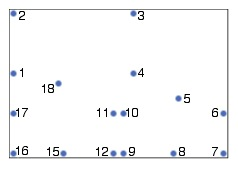
\includegraphics[scale=0.8]{LoudspeakerPositions}}
\caption{{\it Blue points represent the positions of the 16 speakers used in the examples below}}  
\label{Speakers Positions}
\end{figure}

For each pixel of a selected view matrix (of X * Y pixels), the pixel value is set to the  squared amplitude returned by the dbap algorithm as if a source was at this position. The visual result is a picture that shows to the user the spatial response of  a loudspeaker. The lighter pixels are positions where amplitudes are close to 1. and the darker ones, positions where amplitudes are close to 0.. As expected, the more far the source is from the loudspeaker, the less high is the amplitude. However the presence of “digs” in the spatial distribution of the amplitude response illustrates how the dbap algorithm works when a source moves between several loudspeakers. Those graphical informations, even aesthetic there are, give to the user a kind of hitmap that could assist him during space scripting and performing.

\begin{figure}[ht]
\centerline{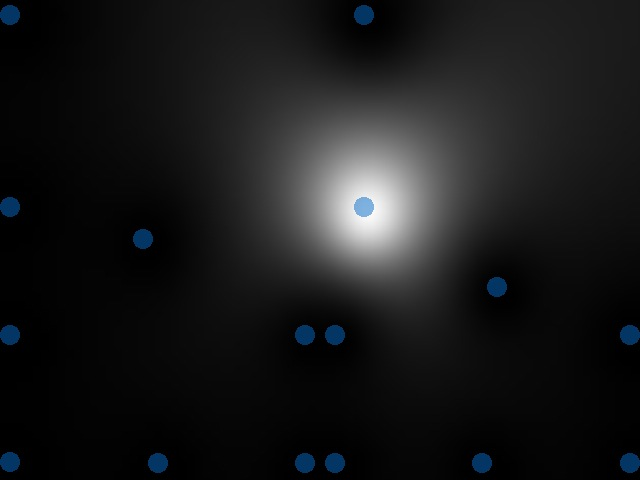
\includegraphics[scale=0.5]{spk4_r_6_b_0}}
\caption{{\it Representation of the levels 2D distribution for speaker 4 - parameter values are 6dB for rolloff, and 0. for blur}}  
\label{Level distribution for one speaker}
\end{figure}

But those pictures of spatial response of each loudspeaker need to be shown together in one visualization. The layout “fusion” method chosen is a max operation between each pixel of each pictures. The graphical result shows straight segmented parts in space corresponding to every spatial influence zones of loudspeakers. Here the darker pixels have to be explain as positions where the source is equal mixed between the closest loudspeakers. The following figures illustrate several settings of rolloff and blur parameters on all loudspeakers. The last picture illustrates a weights preset that keeps only five loudspeakers set with different weights for each of them.

\begin{figure}[ht]
\centerline{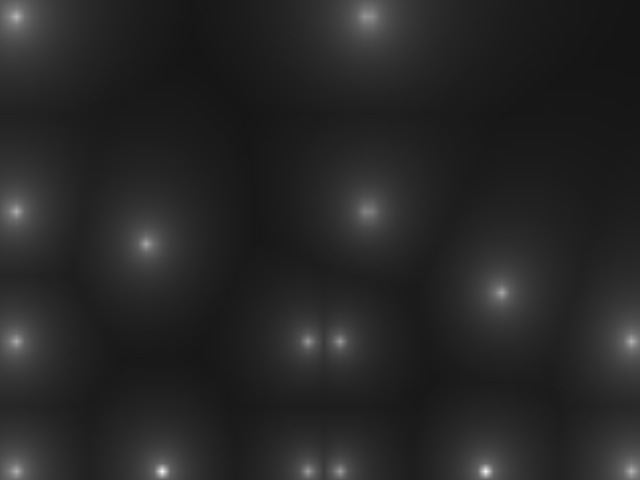
\includegraphics[scale=0.5]{all_r_2_b_0}}
\caption{{\it Representation of the 2D distribution of levels for all speakers - parameter values are 2dB for rolloff, and 0. for blur}}  
\label{Level distribution for all speakers}
\end{figure}

\begin{figure}[ht]
\centerline{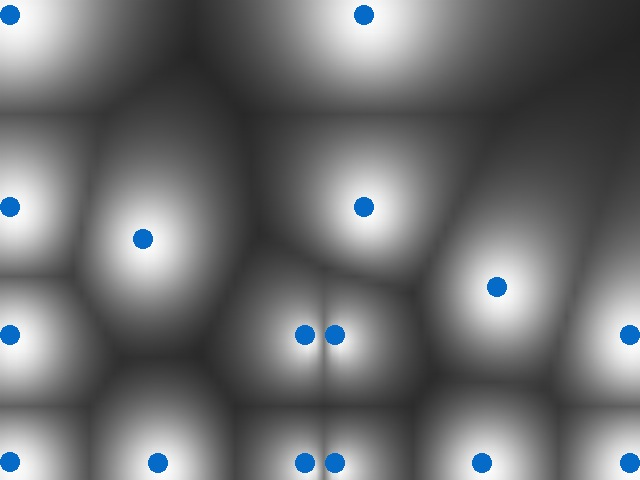
\includegraphics[scale=0.5]{all_r_6_b_0}}
\caption{{\it Representation of the 2D distribution of levels for all speakers - parameter values are 6dB for rolloff, and 0. for blur}}  
\label{Level distribution for all speakers}
\end{figure}

\begin{figure}[ht]
\centerline{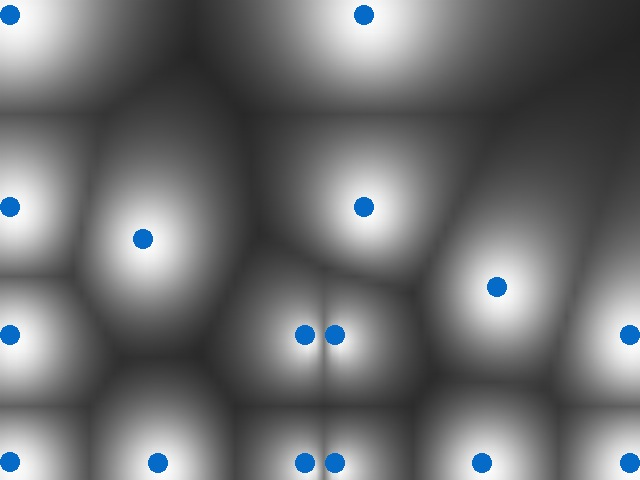
\includegraphics[scale=0.5]{all_r_6_b_0.2}}
\caption{{\it Representation of the 2D distribution of levels for all speakers - parameter values are 6dB for rolloff, and 0.2 for blur}}  
\label{Level distribution for all speakers}
\end{figure}

These pictures can be generated in realtime by the algorithm, and thus be used as an user interface for source positionning, e.g. for mouse interaction, or even better for tactile-screen interaction. 

\section{further development}


\section{Acknowledgements}

Initial development of DBAP was done for the workshop and exhibition ``Living room'' at Galleri KiT in Trondheim, 2003, produced by The Norwegian production Network for Electronic Arts. The initial implementation in C of the DBAP algorithm was done by André Sier. Extensive and valuable feedback has been given by Mathieu Chamagne. 



\bibliographystyle{IEEEtranS}
\bibliography{icmc2009-dbap} % requires file template.bib

\end{document}

%
%This is the template file for the proceedings of the 9$^{th}$ International Conference on Digital Audio Effects (DAFx-06). 
%This template has been generated from WASPAA'99 templates and aims at producing conference proceedings in electronic form. 
%The format is essentially the one used for ICASSP conferences.

%Please use either this \LaTeX{} or the accompanying Word formats when preparing your submission. 
%The templates are available in electronic form at the website:
%\\ \href{http://www.dafx.ca}{http://www.dafx.ca}. Thanks!

%

%
%This template can be found on the conference website.

%\subsection{Figures} 
%All figures should be centered on the column (or page, if the figure spans both columns). 
%Figure captions (in italic) should follow each figure and have the format given in Figure \ref{fft_plot}.
%\begin{figure}[ht]
%\centerline{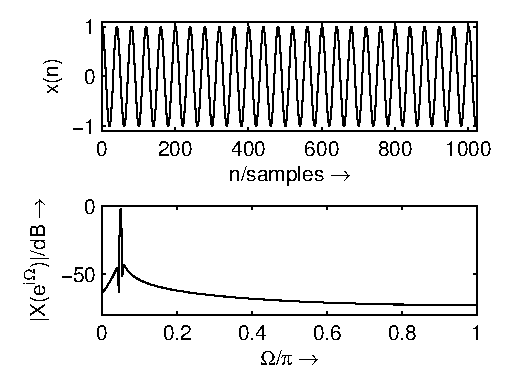
\includegraphics[scale=0.8]{fft_plot2}}
%\caption{{\it Sinusoid in time and frequency domain.}}  
%\label{fft_plot}
%\end{figure}
%Figures must be vectorial (no screen copy, no bitmap, etc). For example when using \texttt{Matlab}, export using either Postscript or PDF format. Also, in order to provide a better readibility, figure text font size should be at list identical to footnote font size. To do so using \texttt{Matlab}, use the \texttt{subplot} command before plotting.

%\subsection{Tables} 
%As for figures, all tables should be centered on the column (or page, if the table spans both columns). 
%Table captions should be in italic, follow each table and have the format given in Table \ref{tab:example}.

%\begin{table}[htdp]
%  \begin{center}
%    \begin{tabular}{|c|c|}\hline
%    	angle ($\theta$, rad) & $\sin \theta$ \\\hline
%	$\frac{\pi}{2}$ & 1 \\
%	$\pi$ & 0 \\
%	$\frac{3\pi}{2}$ & -1 \\
%	$2\pi$ & 0 \\\hline
%    \end{tabular}
%  \end{center}
%  \label{tab:example}
%  \caption{{\it Basic trigonometric values.}}
%\end{table}%

%\subsection{Equations}
%Equations should be placed on separate lines and numbered:

%\begin{equation}
%X(e^{j\Omega})=\sum_{n=0}^{N-1}x(n)e^{-j\Omega n}
%\label{eq1}
%\end{equation}
%where the sequence $x(n)$ in equation (\ref{eq1}) is a windowed frame:
%\begin{equation}
%x(n)=s(n)\cdot w(n)
%\label{eq2}
%\end{equation}
%with a window function $w(n)$.

%\subsection{Page Numbers}
%Page numbers will be added to the document electronically, so {\em please leave the numbering as is},
%that is, the first page will start at page DAFX-1 and the last page, at most, will have to be DAFX-6
%for the submission of papers for an oral presentation or DAFX-4 in the case of a poster presentation.

%\subsection{References}
%The references will be numbered in order of appearance \cite{Mitra:Kaiser:1993:DSP:handbook}, \cite{Haykin:1991:adaptive:filter}, \cite{Moorer:2000:AES:audio:millenium} and \cite{Arfib:1998:DAFx}. Please avoid listing references that do not appear in the text (we did the opposite in this template).

%\subsubsection{Reference Format}
%The reference format is the standard IEEE one. We recommend to use BibTeX to create the reference list.

%\section{Conclusions}
%This template can be found on the conference website. 
%If you wish to include two authors' affiliations please use the companion LaTeX template tmpl\_la2\_href. 
%Please, submit full-length papers (max.~6 pages for oral presentation and max.~4 pages for posters).
% 
%Submission is fully electronic and automated through the Conference Web Submission System. 
%DO NOT send us papers directly by e-mail. 

%\section{Acknowledgements}
%Many thanks to the great number of anonymous reviewers!

%%\newpage
%\nocite{*}
%\bibliographystyle{IEEEbib}
%\bibliography{template} % requires file template.bib

%\end{document}
